\documentclass[a4paper,10pt,twoside]{IEEEtran}

\usepackage{abstract}
\usepackage{algorithm}
\usepackage{algpseudocode}
\usepackage{graphicx}
\usepackage{placeins}
\usepackage{hyperref}
\usepackage{pdfpages}
\usepackage{fullpage}
\usepackage[bf]{caption}
\usepackage[english]{babel}
\usepackage{verbatim}
\usepackage{cite}
\usepackage{wrapfig}
\usepackage[marginpar]{todo}
\usepackage{paralist}
\usepackage{booktabs}
\usepackage{subcaption}
\usepackage{mathtools}
\usepackage{fancyhdr}

\usepackage{tikz}
\usetikzlibrary{calc,intersections}
\usepackage{amssymb}

\hypersetup{
    colorlinks,
    pdftitle={Final Report Option 1 IN4254 Smart Phone Sensing},
    pdfauthor={in4254-dhoepelman-mprovokluit},
}

\setlength{\parindent}{0pt}
\setlength{\parskip}{2ex}

\usepackage[utf8]{inputenc}
\usepackage[T1]{fontenc}

\newcommand{\axis}[1]{$#1$\nobreakdash-axis}
\newcommand{\plane}[2]{$#1#2$\nobreakdash-plane}

\title{\huge{\textbf{Final Report Option 1}\\IN4254 Smart Phone Sensing}}
\date{\today}
\author{David Hoepelman (1521969) \and Mark Provo Kluit (1263099)}

\setlength{\headheight}{15pt}
\addtolength{\headsep}{15pt} % no love between header and main text
%\addtolength{\textheight}{-20pt} % more space between text and empty footer

\pagestyle{fancy}
%\renewcommand{\chaptermark}[1]{\markboth{Chapter\ \thechapter\ #1}{}}
%\renewcommand{\sectionmark}[1]{\markright{\thesection\ #1}{}}
 
\fancyhf{}
\fancyhead[LE,RO]{\thepage}
\fancyhead[RE]{\textit{\nouppercase{\leftmark}}}
\fancyhead[LO]{\textit{\nouppercase{\rightmark}}}
 
\fancypagestyle{plain}{ %
\fancyhf{} % remove everything
\renewcommand{\headrulewidth}{0pt} % remove lines as well
\renewcommand{\footrulewidth}{0pt}}

\begin{document}

\maketitle

\newpage
\pagenumbering{roman}

%% 1: up to sections; 2: up to subsections
%\setcounter{tocdepth}{1}
%\tableofcontents

\newpage
\pagenumbering{arabic}

\section{Basic Information}
\label{sec:basic-information}
The two phones we used are the Samsung Galaxy~S (Mark) running on Android~2.3.3 and LG Nexus~4 (David) running on Android~4.4.3. \autoref{tab:used-libraries} shows the libraries that are used in the application. The ORMLite library is used to store and retrieve data from an SQLite database as Java objects. The Apache Commons Math library is used for computing Eucledian distance, mean and standard deviation. Guava provides various utility functions used by the application.

\begin{table}[ht]
\centering
\caption{Libraries used by the Android app.}
\begin{tabular}{ll}
\toprule
Library & Version\\
\midrule
ORMLite & 4.48\\
Guava & 17\\
Apache Commons Math & 3.2\\
\bottomrule
\end{tabular}
\label{tab:used-libraries}
\end{table}

\section{Activity Monitoring}
\label{sec:activity-monitoring}
\subsection{Technical methods}
We define four activities that need to be recognized by the application: Sitting, Walking, Running, and Jumping.
The application measures the three axes of the accelerometer every 20~ms and groups them together in windows of 240 samples, making the windows 4.8~s long.
We made half of every window overlap, so that (after the first window) every 2.4~s a window can be completed.

For each window several features are computed:

\begin{itemize}
\item Mean $\mu$ for each axis: $\mu_x$, $\mu_y$, and $\mu_z$
\item Standard deviation $\sigma$ for each axis: $\sigma_x$, $\sigma_y$, and $\sigma_z$
\item Correlation between each two axes:  $\text{Corr(}x,y{)}$, $\text{Corr(}y,z{)}$, and $\text{Corr(}z,x{)}$
\end{itemize}

To classify the windows a k-NN classifier was constructed.
The Euclidean distance was used as a distance measurement.
For $k$ we used  $\lceil\sqrt{n}\rceil$, where $n$ is the number of windows in our training database.
We used a random tie-breaker if more than 1 class had the equal (largest) number of neighbours. 

\subsection{Performance evaluation}
We collected 20 windows of each activity type as training and 40 different windows of each activity type as testing data which were fed into our classifier.
The resulting confusion matrix is shown in \autoref{tab:confusion-matrix}.

\begin{table}[ht]
\centering
\caption{Confusion matrix of our classifier.}
\begin{tabular}{lrrrr}
\toprule
& Sitting & Walking & Running & Jumping  \\
\midrule
Sitting & 0.93 &  0.08 &       &       \\
Walking &       & 1.00 &       &       \\
Running &       &  0.10 & 0.75 & 0.15 \\
Jumping &       &        & 0.10 & 0.90 \\
\bottomrule
\end{tabular}
\label{tab:confusion-matrix}
 \end{table}

The confusion matrix shows that the classifier is able to classify activities which reasonable accuracy, especially considering how little training was done.
Running is hardest to classify, which can be explained because the movements often resemble either walking or jumping.

\section{Localization}
\label{sec:localization}

\subsection{Data collection}
\label{sec:loc-localization-method}
For each of the available 17 rooms on the 9$^{\text{th}}$ floor of EWI, we collected Wi-Fi signal strengths of all the access points our mobile phone could find.

The signals collected for training the locator have been collected using the LG Nexus~4 smart phone.
In addition to it being able to detect 5~Ghz WiFi signals, the Samsung Galaxy~S took a much longer time to detect all WiFi signals and had a much worse reception.
In the time that the Nexus~4 could detect the RSS of all visible networks (usually about 20) the Galaxy~S usually had detected only about 2 or 3 networks. While more scans revealed other networks they did not include the previously detected networks.
  
This shows that not all smartphones might be suitable for this task, and that worse results might be achieved if the user does not use a relatively recent and high-end smartphone.

In total we have collected \textbf{3300} scans on 3 different days.
A scan list contains the access points (AP's) that were detected as a list of $signal = (BSSID, SSID, level)$ tuples where $level$ is expressed in dBm with a range of $[-30,-100]$.
Both 2.4~GHz and 5~GHz access points were detected and stored in the database.
Most rooms have either 180 or 240 scans, depending on which days they were accessible.
The collected scans inside a room were evenly divided among the room area.

On average each scan contains 20~$BSSID$'s, although the number varies per room.
We did a fixed number of scans per room on every day, but this does not translate well into a sampling time per cell.
The reason for this is that the time required to perform a signal scan
differs greatly depending on the number of AP's that are visible in a room.

\subsection{Localization}
\label{sec:loc-data}

We chose to use \textbf{Bayesian Filters} for our localization method.
We have drawn a rough not-to-scale map of the rooms, and show it to the user as part of our GUI.
Because Bayesian gives a probability distribution for location, we show the probability of each room in this GUI and give likely (> 50\%) or probable (> 20\%) rooms another color.
See the screenshot in \autoref{fig:screenshot}.

For our calculations we group the training data on $BSSID$ and $Room$ and calculate the normal distribution $N_{BSSID,Room}(\mu_{BSSID,Room}, \sigma^2_{BSSID,Room})$ using the measured signal strengths. We identify an AP using the $BSSID$, because it is guaranteed to be globally unique.

We provide an example with 2 BSSID's and two Rooms, pulled from our collected data.
You can see the histogram of the 4 $(BSSID, Room)$ combination in \autoref{fig:histogram}.
Their respective normal distributions can be seen in \autoref{fig:distribution}.
 You can clearly see that there is a difference in the distributions of the received signal strengths, even though these rooms are next to each other and not separated by a wall.
 This gives high hopes for the effectiveness of the Bayesian filter approach

Signals whose $SSID$ is either ``TUvisitor'', ``tudelft-dastud'',
or ``Conferentie-TUD'' are ignored.
This is because most access points of the TU Delft sent out four different $SSID$'s (the fourth is ``eduroam'') with different $BSSID$'s.
As these signals come from the same physical location and have the same
frequency (and probably the same radio's) we did not think they would add more
information, and at worst might make our results less accurate (by processing
essentially the same signal 4 times, thus biasing the results heavily on those AP's).

For localization we express the location as a probability vector $\mathbf{loc}$, with $\mathbf{loc}_{r}$ being the probability that we are in room $r$. 
We initially start with the \emph{initial belief} where all locations have the same probability $\mathbf{loc}_r = \frac{1}{|\mathbf{loc}|}$.
We then do a WiFi scan which gives a list of signals.
We sort this list on level, with strongest level first.
As long as the largest probability is under a threshold $0.95$ we then iterate the list, while adjusting the location each iteration.
The location is adjusted by getting for each room the chance of that signal level and multiplying it with the existing probability. After each iteration we normalize $\mathbf{loc}$ by making it sum to 1.
\\
\begin{algorithmic}
	\State $scan \gets \text{list of } (BSSID, SSID, level) \text{ sorted on }level$
	\While {$\max\left(\mathbf{loc}\right) < 0.95$}
		\State $signal \gets \text{next}\left(scan\right)$
		\ForAll{$Room$}
			\State $p \gets N_{BSSID,Room}(level-0.5,level+0.5)$
			\State $\mathbf{loc}_{Room} \gets \mathbf{loc}_{Room} \cdot p $
		\EndFor
		\State $\text{normalize}\left(\mathbf{loc}\right)$
	\EndWhile
\end{algorithmic}

$\mathbf{loc}$ is retained between scans until the locator is reset by the user to its initial belief.

\subsubsection{Number of access points}
\label{subsec:loc-numap}

While we achieved a pretty good accuracy with pure Bayesian filters (see performance evaluation section), we had trouble in the \emph{Coffee} room which did not have a large number of APs visible, thus providing too little information for our Bayesian filter.
We solved this problem by constructing $N_{\#,Room}$ distributions.
This distribution gives the probability for number of AP's in a scan based on the $\mu$ and $\sigma$ of the number of AP's per room in the training data.

As can be seen from the average number of APs visible in a room in \autoref{fig:graph-numberAPperRoom} this varies between rooms, and thus can provide extra information for our localization.

We append the following to the previous algorithm:
\\
\begin{algorithmic}
	\If {$\max\left(\mathbf{loc}\right) < 0.95$}
		\ForAll{$Room$}
			\State $p \gets N_{\#,Room}(|scan|-0.5,|scan|+0.5)$
			\State $\mathbf{loc}_{Room} \gets \mathbf{loc}_{Room} \cdot p $
		\EndFor
		\State $\text{normalize}\left(\mathbf{loc}\right)$
	\EndIf
\end{algorithmic}

\subsection{Movement Model}
\label{sec:loc-movement-model}

We tried various approaches for our movement model, see \autoref{sec:innovation}.
We finally settled on re-using our activity classifier as a detector of movement and approximation for the number of steps taken. 
We treated a window classified as sitting as no steps taken and any other window (walking, running or jumping) as 4 steps, because this was about the number of steps we took in the 2.4~s window size.
We tried to make our windows as long as a single step (\~0.65s), but these windows turned out to be too short to provide accurate detection.

Every time the the steps counter detects movement it signals the locator.
The locator then calculates the possible movement area based on a minimum step size of 0.5~m and a maximum step size of 1.2~m.
The probability of every room is then distributed among this area, where the middle of the area is in the center of the room.

This means that a certain part of the room probability remains in that room (the fraction of the "movement"  area that overlaps with the room physical area) while the remaining probability goes to the adjacent rooms (the fraction of the "movement" area that overlaps with the adjacent room physical area).

Due to the size of the rooms (about 7.2~meters for the hallway) and the maximum of 4 steps (4.8~m) probability only has to be distributed among adjacent rooms.

The following algorithm implements this idea:
\begin{algorithmic}
	\State $longest = 1.2 \cdot s$
	\State $shortest = 0.5 \cdot s$
	\State $room\_radius = \frac{7.2}{2}$
	\State $p_{in\_adjacent} = \max\left\{0, \frac{longest - room\_radius}{longest-shortest}\right\}$
	\State $\mathbf{loc'} = \mathbf{0}$
	\ForAll{$Room$}
		
		\ForAll{$a \in Room_{adjacent}$}
			\State $\mathbf{loc'}_a \gets \mathbf{loc'}_{a} + \mathbf{loc}_{Room} \cdot \frac{p_{in\_adjacent}}{|Room_{adjacent}|} $
		\EndFor
		\State $\mathbf{loc}_{Room} \gets \mathbf{loc}_{Room} \cdot (1-p_{in\_adjacent})$
	\EndFor
	\State $\mathbf{loc} \gets \mathbf{loc} + \mathbf{loc'}$
\end{algorithmic}

\subsection{Performance evaluation}
\label{sec:loc-evaluation}

For our performance evaluation we used off-line processing. We divided the scans of our training data into 10 random partitions, and tested every partition while using the other partitions as training data for the locator.

Using this method we achieved an accuracy of \textbf{83\%} (2731 correct out of 3300).
While analyzing the data we saw that a lot of the misclassified scans occurred in the Coffee room,
where a scan usually contains at most three signals. This is not enough for the Bayesian filter.

To alleviate this problem we altered our code to take the number of visible signals into account.
This improved our accuracy to \textbf{89\%} (2945 of 3300).
The technical implementation for this is specified in section \ref{subsec:loc-numap}.
If we mark adjacent rooms as correct too, which is not unreasonable as some training scans were taken on the border between rooms, the accuracy increases to \textbf{95\%} (3132 of 3300).

In \autoref{fig:iterations-needed} the number of iterations that is needed for a certain (95\% certainty) localization is visible.
We see that almost all signals are used, and only after about 23 signals the information is not useful anymore.
We do note that this is purely for the 95\% certainty threshold.
We have not tested how less data or a lower iterations cap would influence the number of correct (but less certain) localizations.

\section{Cloud Computing (1 page)}
\label{sec:cloud-computing}
For cloud computing we decided to implement the ability to spy on the detected localization using a second phone. The ``NSA fragment'' allows another user to see the location of the first user on a map. More precisely, the GUI shows a map -- identical to the map shown in the localization testing GUI -- which duplicates the probabilities shown on the screen of the phone of the first user.

Initially the Google Cloud Messaging (GCM) service was used, but this proved to be quite slow. Because of this reason, we switched to using using a simple direct TCP socket connection. When the user enters an IP address in the GUI of \textsc{LocatorNSAFragment}, the application creates a new \textsc{Thread} which creates a \textsc{ObjectInputStream} from a client socket. It then calls the \textsc{readObject()} method on this object to receive \textsc{Map<Room, Double>} and if Java can successfully deserialize the object, it will use the received probabilities to update the map shown on the screen.

Response time was shown to be much faster; sending the location probabilities from the LG Nexus 4 to the Samsung Galaxy S over the eduroam network takes on average about $1.6$~seconds. Furthermore, the approach using TCP sockets was found to be easier to implement than GCM.

\section{Challenges \& Innovation (0.25 pages)}
\label{sec:innovation}
\subsection{Activity Monitoring Difficulties}
One of the challenges of activity monitoring was selecting the appropriate features and the size of the feature vectors.
We noticed that the correlation features (visually) do not seem to have clear clusters.

Furthermore, it proved to be difficult to reliably classify activities with small windows of around 60 samples. One possible reason is that we used overlapping windows (the latter 30 samples are equal to the first 30 samples of the next window), so there is less difference between two adjacent windows.
This forced us to count steps using windows of 240 samples, which take about 2.5 seconds to collect.
For this reason we estimate that the user has taken four steps when a window is classified as non-sitting.

\subsection{Localization Difficulties}

We did not have major difficulties with implementing the localization.
We were actually surprised at the relative easy and relative good accuracy our Bayesian filter provided.

We did have a lot of problems with implementing our movement model, but did not address them in this report as we were told the movement model should not be in this report.

\autoref{fig:correctness-perroom} shows that room \text{C4\_AISLE4} has an unusually low percentage of correct localizations. Our database shows that in this room \text{C7\_AISLE7} has a 15~\% probability of getting chosen.
We attribute this to a human error during training, as all the incorrectly localized scans are done within a few minutes of each other.
In short we once selected the wrong room while collecting the training data.

\section{Individual Workload (0.25 pages)}
\label{sec:individual-workload}
David:
\begin{itemize}
    \item Activity training
    \item Activity measurement window collection
    \item Computation of feature vectors
    \item Bayesian locator
    \item Offline processing of Wi-Fi measurements
    \item NSA functionality
    \item ORMLite database code
    \item SQL queries and figures generation for reports
\end{itemize}

Mark:
\begin{itemize}
    \item Activity testing
    \item k-NN classifier
    \item Wifi measurement window collection
    \item Steps counter and movement model in Bayesian locator
    \item Localization training \& testing maps
    \item General bug fixes and some reliability and performance improvements
\end{itemize}

\section{Possible Future Directions (0.25 pages)}
\label{sec:future-directions}
\subsection{Activity Monitoring}
For activity monitoring we might be able to improve the classification by using the Mahalanobis distance instead of the Euclidean.

\subsection{Localization}
Bayesian filters are not that useful if you have rooms with only a low number of visible access points.
Our trick to take the number of AP's into accounts works well when there
are not too many rooms with few visible AP's.
However, if there are more rooms like the Coffee room, this approach will likely fail.
Another possibility we contemplated was to create a bitstring of present/not-present $BSSID$'s for the current scan and the training data.
Computing the hamming distances to the training data points increases the amount of information that
is available to the filter, thus possibly increasing the accuracy.
This will more likely work in the general case.

%\clearpage
%\phantomsection
%\addcontentsline{toc}{chapter}{References}
%% styles: abbrv, ieeetr, plain
%\bibliographystyle{ieeetr}
%\bibliography{report}

\newpage
\appendix

%\chapter{Source Code}
\label{sec:app-source-code}
TODO

\section{Localization Data}

\begin{figure}[h!]
  \centering
    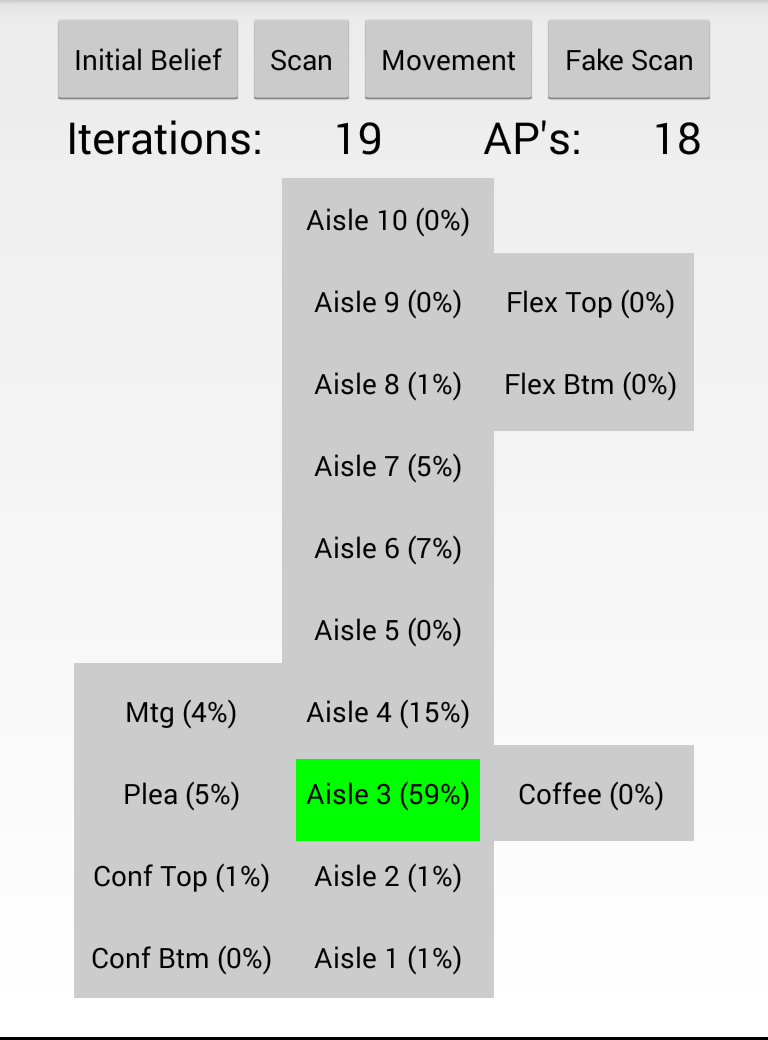
\includegraphics[width=0.36\textwidth]{screenshot}
    \caption{GUI showing successful localization.}
    \label{fig:screenshot}
\end{figure}

\begin{figure}[h!]
  \centering
    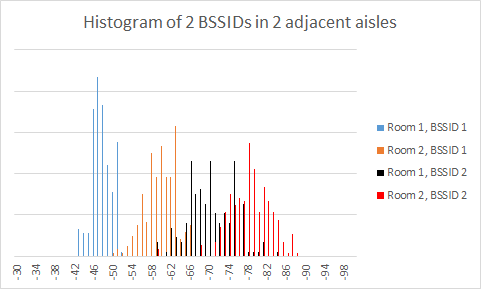
\includegraphics[width=0.5\textwidth]{histogram}
    \caption{Histogram of two BSSID's in two adjacent aisles.}
    \label{fig:histogram}
\end{figure}

\begin{figure}[h!]
  \centering
    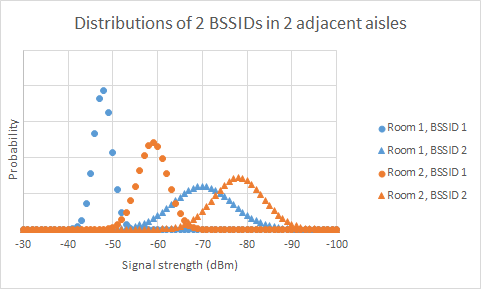
\includegraphics[width=0.5\textwidth]{distribution}
    \caption{Distribution of two BSSID's in two adjacent aisles.}
    \label{fig:distribution}
\end{figure}

\begin{figure}[h!]
  \centering
    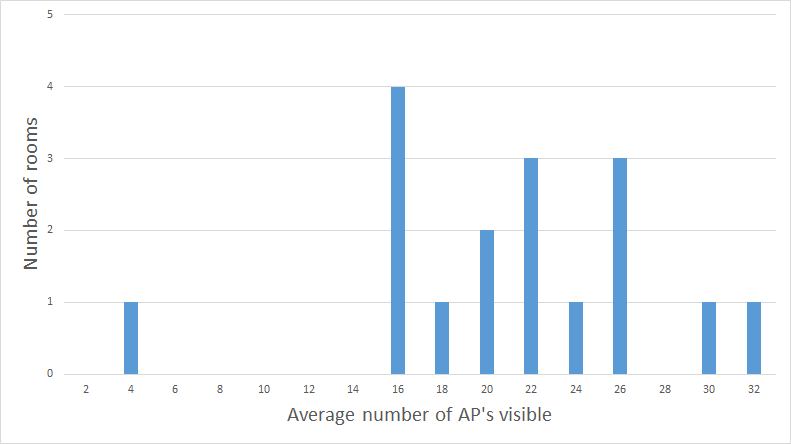
\includegraphics[width=0.5\textwidth]{graph-numberAPperRoom}
    \caption{Number of access points per room.}
    \label{fig:graph-numberAPperRoom}
\end{figure}

\begin{figure}[h!]
  \centering
    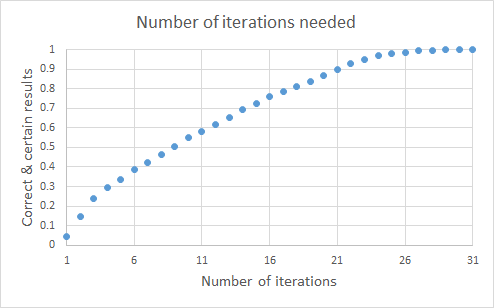
\includegraphics[width=0.5\textwidth]{iterations_needed}
    \caption{Percentage of results that will eventually be correct and certain after a specific number of iterations.}
    \label{fig:iterations-needed}
\end{figure}

\begin{figure}[h!]
  \centering
    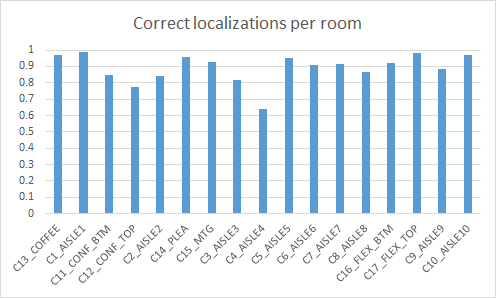
\includegraphics[width=0.5\textwidth]{correctness_perroom}
    \caption{Correct localizations per room when taking the probability of number of AP's per room into account.}
    \label{fig:correctness-perroom}
\end{figure}

\end{document}
